\chapter{Testing, Analysis and Bench-marking; Closing Remarks, Potential Future Work}
\label{cha:Closing}

\section{A Note on Messages and Failures in WL} \label{closing:messages}

If WL is to a be a systems engineering language, it makes sense for error cases, failures, to be readily machine readable and conceived of as input for processing in an automated manner, rather than messages that direct a human user of Mathematica Desktop. This shift is apparent in the recommendation for usage of Failure[] rather than the symbol, \lstinline+$Failed+, simply "a special symbol returned by certain functions when they cannot do what they were asked to do." \cite{noauthor_failedwolfram_nodate}

Opposite this, Failure[], introduces more functionality and information, especially the failure type: "Failure[\textit{"tag"},\textit{assoc}] represents a failure of a type indicated by \textit{tag}, with details given by the association assoc." \cite{noauthor_failurewolfram_nodate} This introduces the potential for an abstract way to handle a failure based on type, programmatically, rather than a specific directive.

A basic example of a Failure object is \lstinline+Failure["InvalidInput", <||>]+, without an association even. Inside the Mathematica frontend it is rendered as in figure \ref{fig:simple-failure}.

\begin{figure}[h]
    \centering
    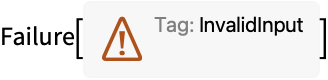
\includegraphics[scale=0.5]{images/closing/O_4.png}
    \caption{A simple Failure object rendered in Mathematica \cite{noauthor_failurewolfram_nodate}}
    \label{fig:simple-failure}
\end{figure}

A more complicated example in terms of metadata and parameterized messaging is generated by the WL code \lstinline$Failure["ExternalOperation", <\|
  "MessageTemplate" -> "External operation `1` failed.", 
  "MessageParameters" -> { "file upload"}\|>]$ and rendered as in figure \ref{fig:templated-failure}.

\begin{figure}[h]
    \centering
    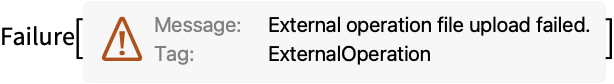
\includegraphics[scale=0.5]{images/closing/O_6.png}
    \caption{A Failure object using a template with positional parameters \cite{noauthor_failurewolfram_nodate}}
    \label{fig:templated-failure}
\end{figure}

Failure can also contain index-able metadata that might be helpful for programmatic retrieval in the failure case. \cite{noauthor_failurewolfram_nodate} In any case, Failure objects can be returned by functions to indicate that an operation did not succeed as expected. This approach allows for more structured error handling, where the calling code can inspect the Failure object to determine the cause of the error and decide how to proceed: They are particularly useful in functional and symbolic programming patterns prevalent in WL, enabling a more nuanced handling of errors compared to traditional imperative error handling mechanisms like throwing exceptions.

Similarly, Message \cite{noauthor_messagewolfram_nodate} is about signaling that something unusual has occurred during the evaluation of an expression - where Failure is a way to encapsulatively represent the occurrence of an error and carry forward information about that error in a structured form, a function might generate a Message to inform the user of an error and then return a Failure object to programmatically indicate the error condition to the calling code.

When a Message is generated, it does not by itself halt execution; the computation continues unless the message is associated with an error severe enough to trigger a termination of the evaluation. \cite{noauthor_messagewolfram_nodate} Messages can be controlled and manipulated using functions like Off, On, and Quiet, allowing to suppress or enable specific messages. This is useful for managing the verbosity of output during computation, especially in cases where certain warnings or errors are expected and do not necessarily indicate a critical failure.

A production code example with messaging has already been shown in section \ref{pattern-matching-implementation-example} on the production code example: the final version uses messaging to ensure communication beyond the \lstinline+$Failed+ return symbol, combining the old trend of its usage with the more modern messaging functionality, a common practice when not replacing with Failure. 

Usage messages are a way to document the purpose and usage of symbols (typically functions) directly within the WL environment. These messages provide brief descriptions of what a function does, its arguments, and sometimes examples of how to use it. Usage messages are helpful for both package developers and users, as they offer immediate, inline documentation accessible through the WL interface. They are also used in the present package, see near the top of the source code in Appendix \ref{app:Source}.

Testing in WL therefor involves evaluation strategies that check for Messages or Failures in the modern case. To this end, the language offers a suite of testing functionality: for example, VerificationTest fails by default if any Message is issued (unless it is told to expect a message, e.g. of a certain type).

\section{Testing in Wolfram Language}


\section{Testing Approach for this Project}

 The guiding principle during development of this project was testing  throughout, by manually checking the output PDF representation of the \LaTeX code against the transformed WL notebook, with a variety of documents taken from the day-to-day at RISC. Two main failure cases were discovered, Unknown Pattern Failures and Incompleteness Failures, which will be outlined below after a note on the implemementation of the WL testing framework discussed above.

 \subsection{Test Framework Implementation for this Project}



 \subsection{Unknown Pattern Failures}

 the central parseNotebookContent[] (parseTmaEnv[]) recursive function was called with an expression that did not fit any of the expected patterns, falling into the most generic case, cf. Snippet \ref{prog:parseNotebookContent[other_]}, for the relevant parseNotebookContent[] line.

 \begin{program}
\caption{Notebook source code for a simple math formula.}
\label{prog:parseNotebookContent[other_]}
\begin{LaTeXCode}
parseNotebookContent[other_] := StringJoin["\\textcolor{red}{", "Pattern not found! ", ToString[other], "}"]
\end{LaTeXCode}
\end{program}

The manually verifiable output follows the screenshot presented in Image \ref{fig:parseNotebookContent[other_]-output}. Also visible is the run-on output of the string representation of the unmatched pattern printed to the underlying \LaTeX. (The grayed out "Cell reached" and similar directives are used for cross-referencing navigation in the output document back with the origin-document.)

\begin{figure}[h]
    \centering
    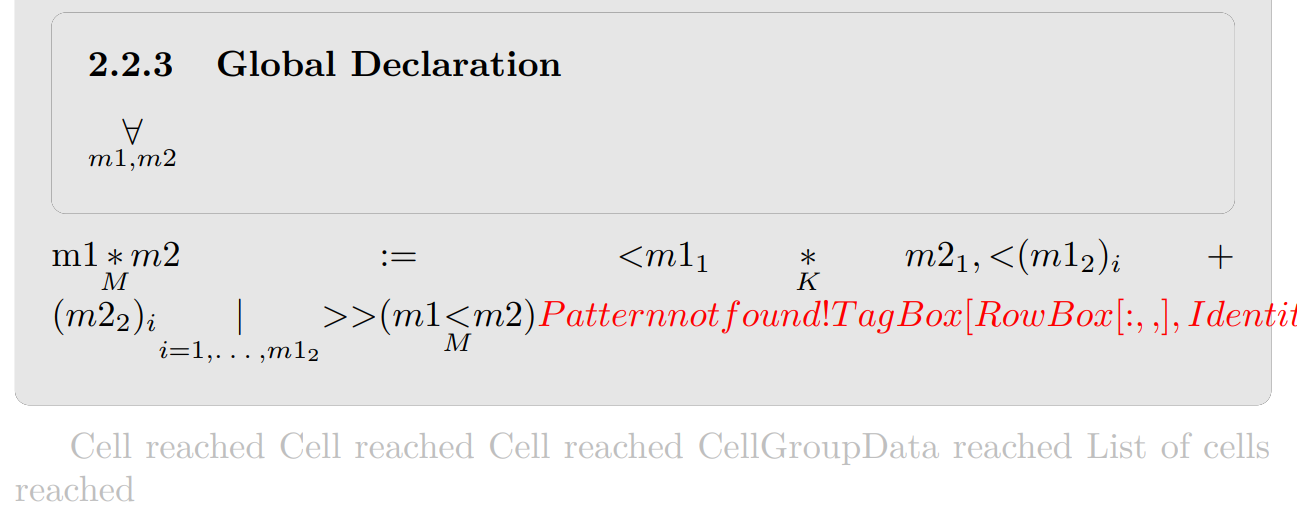
\includegraphics[scale=0.5]{images/closing/Screenshot 2024-03-08 171539.png}
    \caption{parseNotebookContent[other\_] output in document with \LaTeX command formatting}
    \label{fig:parseNotebookContent[other_]-output}
\end{figure}

[TODO: Messaging and connect to Testing Framework.]

\subsection{Incompleteness Failures}

Tests for incompleteness are trickier in that they can only, at least as far as this project without AI/LLM-based approaches is concerned, be checked manually against the original notebook. This kind of testing formed the basis for development.
 
 
\section{Analysis and Review}

\subsection{Analysis}

\subsection{Review}


\section{Closing Remarks: Wolfram Language as a Software Engineering Tool and Integrating with Other Languages and Environments, Potential Future Work}

\subsection{Using Wolfram Language for Software Engineering}

[Insights into working with WL would prob. be nice, also integrations into and of other languages and environments interesting.]

\subsection{Potential Future Work}

[Future Work Ideas? Wolfram Cloud Object refinement maybe.]

Currently WL and Theorema Language level typesetting cutomizations are required to be registered to the package (via a public package variable) and also custom-specified in the \LaTeX template. Since the latter part will always be required, one idea for further simplification (at the possible cost of less explicit control over the transformation rules) is to make the template the leading file and find the customization rules based on string pattern-matching, taking care of registration to the package variable dynamically and in the background. This improvement would be a convenience to the user.